\chapter{Sputtering of Nanowires}


\section{First results in $Mn$ irradiated $GaAs$}

Introduction by Mn in GaAs (JPhysD)


\section{Simulation results}
\label{sec:simsputering}


Xe, Ar in Si NW: Energy and Diameter dependent SY

The Gaussian ellipsoid approximation to the recoil Profile from SRIM was found as \cite{bobes_ion_2012}



\section{Redeposition}

While irradiating a nanowire standing perpendicular on a substrate as shown in \ref{} material will also be sputtered from the substrate. Some of the sputtered material from the substrate will be redeposited on the nanowire, so that the observable sputter yield will be lower than the actual sputtering. Consider the situation shown in figure \ref{redeposit}. An ion hits the substrate at point A. A possible path of a sputtered atom is indicated by the red line to a point on the nanowire, redepositing the substrate atom on the nanowire. 

\begin{SCfigure}
	\centering
		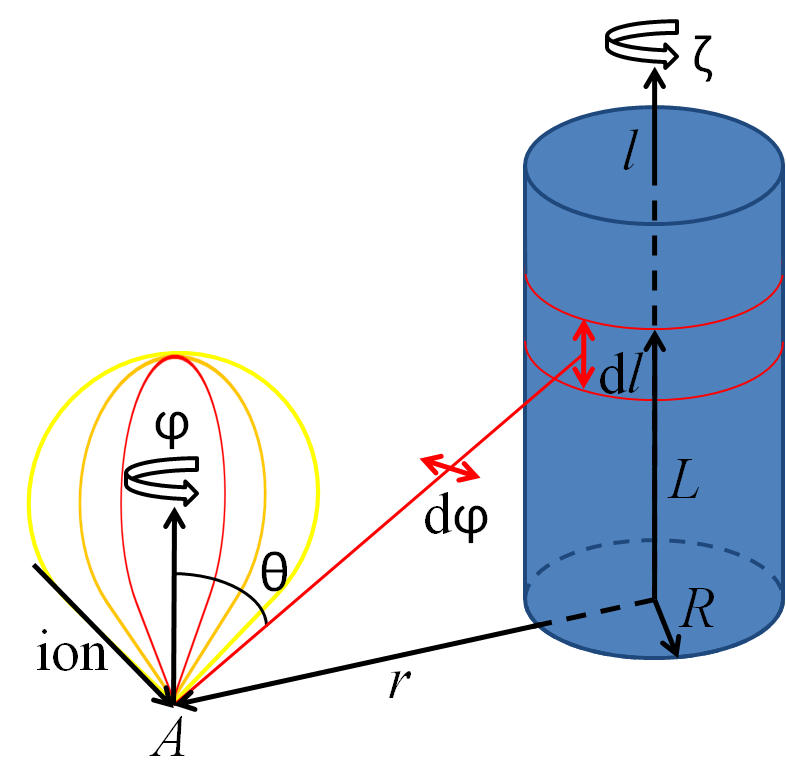
\includegraphics[width=.48\textwidth]{images/redeposit.jpg}
	\caption{} 
	\label{redeposit}
\end{SCfigure}

The following calculation will estimate how large the redeposition is by first calculating the probability of a sputtered atom to hit the nanowire $P$:

\begin{equation}
\label{prob1}
P = \int_0^{2\pi} \! \,\int_0^{\pi/2} \!\! H(\theta,\varphi,r,R,L) \, \tilde{SY}(\theta,\varphi) \,cos(\theta)\,\mathrm{d}\theta \, \mathrm{d}\varphi.
\end{equation}

Where $H(\theta,\varphi,r,R,L)$ is the probability distribution of hitting the nanowire. It is $1/(4\pi)$ if the trajectory along $\theta$ and $\varphi$ from $r$ hits the nanowire with length $L$ and radius $R$, and zero otherwise. For irradiation at an angle, the angle distribution of the sputter yield $\tilde{SY}(\theta,\varphi)$ is expected to have a preferential direction along the ion beam \cite{verdeil_angular_2008}. However, the effective distribution becomes rotationally symmetric (independent of the angle $\varphi$) if one neglects the shadowing of the ion beam on the substrate, as all points around the wire are irradiated and the wire is rotated around its axis (angle $\zeta$). This means that a rotationally symmetric angle distribution $\tilde{SY}(\theta)$ of the sputtered atoms from the substrate can be used, as indicated by the yellow, orange and red bulbs. A $cos^\kappa(\theta)$ distribution is chosen, as it forms flattened angle distributions for $\kappa < 1$, which can emulate the rotation of a slanted angle distribution: 

\begin{equation}
\tilde{SY}(\theta) = \frac{SY \cdot cos^\kappa(\theta)}{\int_0^{2\pi} \! \mathrm{d}\tilde\varphi \,\int_0^{\pi/2} \! cos^\kappa(\tilde\theta) cos(\tilde\theta)\,  \mathrm{d}\tilde\theta} \, = SY /c(\kappa) \cdot cos^\kappa(\theta) ,
\end{equation}

where the denominator $c(\kappa)$ normalizes the angle distribution function $cos^\kappa(\theta)$ and $SY$ is the total sputter yield from the surface. The parametrization of $H(\theta,\varphi,r,R,L)$ in $\varphi$ is straightforward, as the integration bounds for $\varphi$ are $[-\gamma, \gamma]$ with $\gamma = arcsin(R/r)$ the angle between $r$ and the tangent to the nanowire in figure \ref{anglesredepo} a). To solve the integration over $\theta$ it is useful to express the distance $q$ from the impact point to the base of the nanowire can be expressed as a function of $\rho = R/r, r$ and $\varphi$:

\begin{equation}
q(\rho,r,\varphi) = r\cdot \sqrt{1 + \rho^2 - 2sin^2(\varphi) - \sqrt{cos^2(\varphi)(cos(2\varphi) - 1 + 2\rho^2)}},
\end{equation}

\begin{figure}
	\centering
		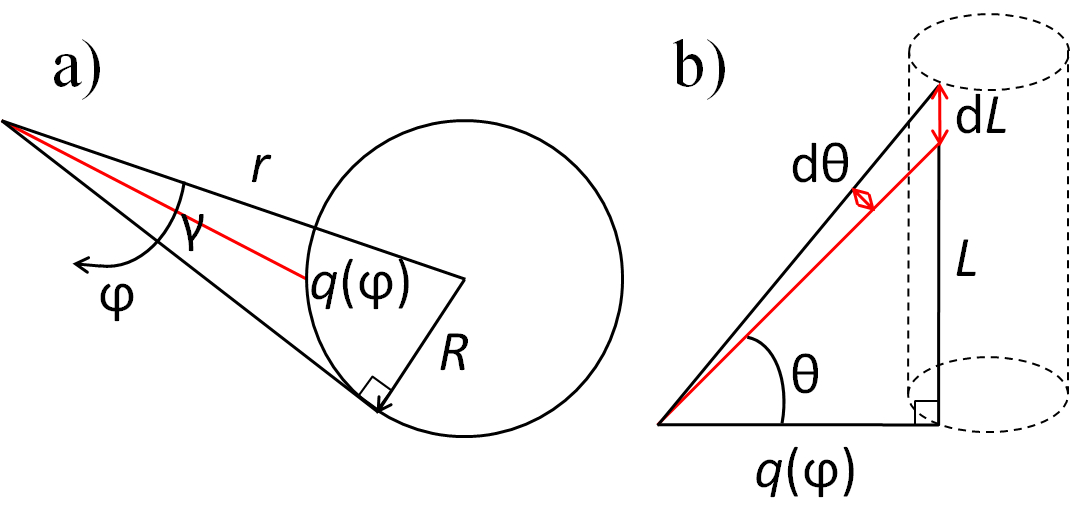
\includegraphics[width=.6\textwidth]{images/anglesredeposition.jpg}
	\caption{Trajectories of a $10\,eV$ $Si-Si$ collision for a) Moliére and b) $Si-Si$ potential. The trajectories end after the same elapsed time for each impact parameter p. Adapted from \cite{eckstein_computer_1991}.}
	\label{anglesredepo}
\end{figure} 

to be able to substitute the integration over $\theta$ by an integration over the length of the nanowire $l$. The substitution can be found looking at figure \ref{anglesredepo} b):

\begin{align*}
\mathrm{d}\theta &= \frac{sin(\theta)}{\sqrt{L^2 + q^2}}\,\mathrm{d}L\\
\theta &= arctan(L/q)
\end{align*}

Inserting into equation \ref{prob1} and simplifying yields:

\begin{equation}
\label{prob2}
P = \frac{2\,SY}{c} \int_0^{\gamma} \! \int_{L_1}^{L_2} \!  \frac{l\,q^{\kappa+1}}{(l^2 + q^2)^{(\kappa + 3)/2}}.
\,\mathrm{d}l \, \mathrm{d}\varphi.
\end{equation}

With $l^*=L_1-L_2$ the area hit on the nanowire is now $\pi \, R \, l^*$, positioned at the height $L= (L_1+L_2)/2$ as indicated between the two red lines in figure \ref{redeposit}. Integrating the probability $P$ to hit the nanowire at each substrate position over the whole substrate area and normalizing it to the area of the nanowire which is hit yields the number of atoms $N$ hitting the nanowire per fluence $\Phi$:

\begin{equation}
\label{prob2}
N/\Phi = \frac{2\,SY}{c \pi Rl^*} \int_0^{2\pi}\! \mathrm{d}\zeta \int_R^{\infty} \!
\int_0^{\gamma} \! \int_{L_1}^{L_2} \! r \frac{l\,q^{\kappa+1}}{(l^2 + q^2)^{(\kappa + 3)/2}}\,\,\mathrm{d}l \, \mathrm{d}\varphi\,\mathrm{d}r \, .
\end{equation}




\section{$Si$ nanowire sputtering by $Ar^+$ irradiation}
\label{sec:sisputtering}